\section{Theoretical Foundations}
\label{sec:Theoretical_Foundations}
In this experiment the Planck constant $h$ was determined. This is a physical constant that relates the frequency of a photon to the energy it carries. This section summarizes the theory and formulas necessary to understand the following experiments on ultrasound in section \ref{sec:Evaluation}.

%-------------------------------------------------------------------------------------------
\subsection{Electromagnetic Radiation}
\label{subsec:Electromagnetic_Radiation}
The various effects that occur during the propagation and interaction of electromagnetic radiation with material objects can be classified into wave and particle phenomena:

\textbf{Wave Phenomena:} Interference and diffraction are described by the wave theory of electromagnetic radiation. From this point of view, the radiation occurs in the form of electromagnetic waves, which can be represented by a continuous wave function \cite{light_quantum}.

\begin{equation}
c = \lambda\cdot f
\label{eq:wave_length_frequency}
\end{equation}
where:
\begin{multicols}{2}
	\begin{center}
		\begin{conditions}
			c & speed of light in $\,^{\text{m}}\!/_{\text{s}}$ \\
			\lambda & wave length in m
		\end{conditions}
		\begin{conditions}
			f & frequency in Hz
		\end{conditions}
	\end{center}
\end{multicols}

\textbf{Particle Phenomena:} Emission and absorption are described by the quantum theory of electromagnetic radiation. From this point of view, the radiation occurs in the form of photon current $\gamma$ (also called light quantum), which interacts with single atoms, electrons etc. in individual quantum processes. This is subject to chance, which is why only probability statements can be made \cite{light_quantum}.

\begin{equation}
E_\gamma = h\cdot f = h\cdot\frac{c}{\lambda}
\label{eq:energy_particle}
\end{equation}
where:
\begin{multicols}{2}
	\begin{center}
		\begin{conditions}
			E_\gamma & photon energy in J \\
			h & Planck constant in J$\cdot$s \\
			f & frequency in Hz
		\end{conditions}
		\begin{conditions}
			c & speed of light in $\,^{\text{m}}\!/_{\text{s}}$ \\
			\lambda & wave length in m
		\end{conditions}
	\end{center}
\end{multicols}

Energy and impulse exchange between radiation and matter can only take place in such quanta. Equation \ref{eq:energy_particle} shows that the magnitude is essentially determined by the Planck constant $h$ (also known as Planck's quantum of action) \cite{light_quantum}.

Since the 20\textsuperscript{th} May 2019 the value of the Planck constant $h$ is exactly
\begin{equation}
h = 6.626\ 070\ 15 \cdot 10^{-34}\ \si{J}\cdot\si{s}.
\label{eq:plank_constant}
\end{equation}
The value of the Planck constant $h$ has been fixed due to the redefinition of the kilogram \cite{planck_constant}.

The two illustrative models are in principle incompatible. On the one hand the wave, the most smudgy thing there is. On the other hand the particle, the most concentrated thing there is. The solution to this dilemma is known as wave-particle duality, which is a concept in quantum mechanics. It expresses the inability to fully describe the behavior of quantum-scale objects with the classical concepts \flqq wave\frqq\ or \flqq particle\frqq\ \cite{light_quantum, wave_particle_duality}.

\newpage
%-------------------------------------------------------------------------------------------
\subsection{Photoelectric Effect}
\label{subsec:Photoelectric_Effect}
The photoelectric effect is the absorption of light quanta by atoms, molecules or solids, in which the photon disappears and transfers part of its energy to an electron. In the case of atoms and molecules, free electrons with kinetic energy $E_k = E_\gamma - E_B$ are formed in the first moment, which can then attach themselves to other particles. $E_B$ is the binding energy of an electron. However, the atoms involved in the process are much heavier, so the energy of these electrons can be neglected. In the case of interaction with solids, a distinction is made between the outer photoelectric effect and the inner photoelectric effect \cite{light_quantum}.

%-------------------------------------------------------------------------------------------
\subsubsection{Outer Photoelectric Effect}
\label{subsubsec:Outer_Photoelectric_Effect}
The light quanta knock photoelectrons out of the surface of metals, metal oxides and semiconductors. To release an electron, its binding energy has to be expended. This binding energy is called the electron work function $W_a$. The photo energy $E_\gamma$ must be at least equal to the electron work function $W_a$ for this effect to occur. The process takes in a thin surface layer place, which corresponds to the penetration depth of the photons. Therefore, the photoelectrons suffer different energy losses and leave the surface with variable kinetic energy \cite{light_quantum}.

\begin{equation}
\widehat{E}_k = E_\gamma - W_a = h\cdot f - W_a
\label{eq:outer_photoelectric_effect}
\end{equation}
where:
\begin{multicols}{2}
	\begin{center}
		\begin{conditions}
			\widehat{E}_k & max. kinetic energy in eV \\
			E_\gamma & photon energy in eV \\
			W_a & electron work function in eV
		\end{conditions}
		\begin{conditions}
			h & Planck constant in J$\cdot$s \\
			f & frequency in Hz
		\end{conditions}
	\end{center}
\end{multicols}

Equation \ref{eq:outer_photoelectric_effect} shows the calculation of the maximum value of this kinetic energy. The electron work function is a surface property and only material-specific at extremely high purity. Absorbed contaminants such as gases, oxide films and other impurities can change the value significantly.Layers used to convert radiation into a photoelectron stream are called photocathodes. If such a layer is combined with a multiplier (resulting in a photomultiplier) a very sensitive radiation detector is obtained \cite{light_quantum}.

%-------------------------------------------------------------------------------------------
\subsubsection{Inner Photoelectric Effect}
\label{subsubsec:Inner_Photoelectric_Effect}
The light quanta that penetrate a semiconductor prodce additional charge carriers. It can be distinguished between photoconductors and photodiodes \cite{light_quantum}.

\textbf{Photoconductors:} When irradiated, the charge carrier density and thus the conductivity increase. This is why they are sometimes also called photo resistors \cite{light_quantum}.

\textbf{Photodiodes:} In the region of the p-n junction, the absorbed photons generate electron-hole pairs. Without an external source, the p-side is positively charged and the n-side is negatively charged, resulting in a photovoltage. This photovoltag can be as high as the diffusion voltage $U_d$. A corresponding current flows under load. Solar cells use this element operation. If an external voltage is applied in the reverse direction, a photocurrent flows in this direction. This current is proportional to the incident radiant power. This diode operation is used for photodetectors. The described processes only take place when the photon energy exceeds a material-specific threshold value, which is the release of an electron bound to the crystal lattice \cite{light_quantum}.

\newpage
%-------------------------------------------------------------------------------------------
\subsection{Counter-Field Method (Millikan)}
\label{subsec:Countervailing_Field_Method}
The counter-field method can be used to determine the kinetic energy of the photoelectrons. Figure \ref{fig:millikan} displays this graphically. The photocathode $K$ to be investigated and the anode $A$, which serves as a collector for the photoelectrons, are located in an evacuated glass bulb. The electrons triggered by monochromatic light of wavelength $\lambda$ have a maximum kinetic energy as shown in equation \ref{eq:outer_photoelectric_effect} \cite{light_quantum}.

\begin{figure}[H]
	\centering
	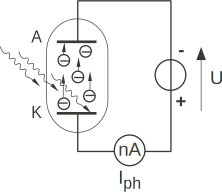
\includegraphics[scale=2]{millikan}
	\caption{This figure shows how the counter-field method is used to determine the kinetic energy of the photoelectrons. The voltage $U$ is increased until the current $I_{ph}$ reaches zero. As soon as the current $I_{ph} = 0$, the voltage $U$ must be equal to the voltage $U_{KA}$ \cite{light_quantum}.}
	\label{fig:millikan}
\end{figure}

If the voltage between anode and cathode is positive, the electrons are still accelerated and the full photocurrent flows, determined by the incident radiation power. If an increasing countervoltage $U$ is applied, fewer and fewer electrons reach the anode until the photocurrent finally disappears at the critical countervoltage $U_o$. Due to the material-dependent contact potential $U_c$ that is present even without an external voltage between cathode and anode, the following equation \ref{eq:millikan} applies for zero photocurrent \cite{light_quantum}.

\begin{equation}
\widehat{E}_k = e\cdot (U_o - U_c)
\label{eq:millikan}
\end{equation}
where:
\begin{multicols}{2}
	\begin{center}
		\begin{conditions}
			\widehat{E}_k & max. kinetic energy in eV \\
			e & elementary charge ($\approx 1.602\cdot 10^{-19}\ \si{C}$)
		\end{conditions}
		\begin{conditions}
			U_o & critical counter-voltage in V \\
			U_c & contact potential in V
		\end{conditions}
	\end{center}
\end{multicols}

\newpage
%-------------------------------------------------------------------------------------------
\subsection{Light-Emitting Diode (LED)}
\label{subsec:light-emitting_diode}
The luminous emission of LEDs is caused by the fact that electrons pass from the conduction energy band to the valence energy band. This means that the electrons change from a higher to a lower energy state. In a regular diode this energy is dissipated as heat. In the case of a light-emitting diode, on the other hand, it is mostly released as light. Figure \ref{fig:led} shows this graphically. This process is the reversal process to the inner photoelectric effect \cite{light_quantum}.

The relationship between the photon energy and the characteristic curve of an LED is given by equation \ref{eq:led}. The diffusion voltage $U_d$ depends on the material, its doping and the geometric structure of the diode. Due to the fact, that light emitting diodes are highly doped, the Fermi energies are close to the band edges and $e\cdot U_d$ is approximately equal to the band gap $E_g$ (usually a little bit smaller). $U_d$ roughly corresponds to the threshold voltage $U_K$ of the characteristic curve. Therefore, equation \ref{eq:led_threshold} can be used as an approximation for the measurable threshold voltage and the wavelength of the emission of an LED \cite{light_quantum}.

\begin{equation}
e\cdot U_K \approx E_\gamma
\label{eq:led}
\end{equation}
thus:
\begin{equation}
U_K \approx \frac{h}{e}\cdot\frac{c}{\lambda}
\label{eq:led_threshold}
\end{equation}
where:
\begin{multicols}{2}
	\begin{center}
		\begin{conditions}
			U_K & LED threshold voltage in V \\
			E_\gamma & photon energy in eV \\
			e & elementary charge ($\approx 1.602\cdot 10^{-19} \si{C}$)
		\end{conditions}
		\begin{conditions}
			h & Planck constant in J$\cdot$s \\
			c & speed of light in $\,^{\text{m}}\!/_{\text{s}}$ \\
			\lambda & wave length in m
		\end{conditions}
	\end{center}
\end{multicols}

\begin{figure}[H]
	\centering
	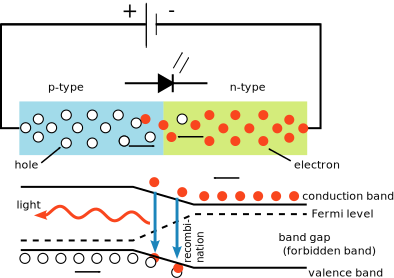
\includegraphics[scale=1.2]{led}
	\caption{Graphical representation of the inner workings of an LED. The p-n junction emits light when electrons cross it. The free electrons move from the conduction band to the valence energy band (lower energy level). To recombine the electrons and the holes, some portion of the energy is dissipated in the form of heat and light (release of photons) \cite{led}.}
	\label{fig:led}
\end{figure}
